\documentclass{beamer}
\usepackage{lmodern}
\usepackage[T1]{fontenc}
\beamertemplatenavigationsymbolsempty
\title[]{Visualisierung komplexer Datenstrukturen}
\subtitle{Dozentin: Carmen van Meegen}
\author[]{Yannick Miguel, Kjell Noack, Florian Schürenberg, Jacqueline Link}
\date[27.02.2024]{27. Februar 2024}
\setbeamercovered{transparent}
\usepackage[backend=biber]{biblatex}
\usepackage{graphicx}
\usepackage{booktabs}
\usetheme{Boadilla}
%\definecolor{myOrange}{rgb}{0.110,0.199,0.45}                   
%\usecolortheme[RGB={110,199,45}]{structure}  
\useinnertheme{rounded}
\usepackage{tikz}
\setbeamertemplate{caption}[numbered]
\addbibresource{Quellen.bib}



\setbeamertemplate{footline}{%
	\leavevmode%
	\hbox{%
		\begin{beamercolorbox}[wd=.333333\paperwidth,ht=2.25ex,dp=1ex,left]{author in head/foot}%
			\usebeamerfont{author in head/foot}\insertshortauthor
		\end{beamercolorbox}%
		\begin{beamercolorbox}[wd=.333333\paperwidth,ht=2.25ex,dp=1ex,center]{title in head/foot}%
			\usebeamerfont{title in head/foot}\insertshorttitle
		\end{beamercolorbox}%
		\begin{beamercolorbox}[wd=.333333\paperwidth,ht=2.25ex,dp=1ex,right]{date in head/foot}%
			\usebeamerfont{date in head/foot}\hspace*{2em}
	\end{beamercolorbox}}%
	\vskip0pt%
}

\begin{document} 
	\begin{frame}
		\maketitle
	\end{frame}        
	\begin{frame}
		\frametitle{Inhaltsverzeichnis}
		\tableofcontents
	\end{frame}
	\addtocounter{framenumber}{-2}
	\setbeamertemplate{footline}{%
		\leavevmode%
		\hbox{%
			\begin{beamercolorbox}[wd=.333333\paperwidth,ht=2.25ex,dp=1ex,left]{author in head/foot}%
				\usebeamerfont{author in head/foot}\insertshortauthor
			\end{beamercolorbox}%
			\begin{beamercolorbox}[wd=.333333\paperwidth,ht=2.25ex,dp=1ex,center]{title in head/foot}%
				\usebeamerfont{title in head/foot}\insertshorttitle
			\end{beamercolorbox}%
			\begin{beamercolorbox}[wd=.333333\paperwidth,ht=2.25ex,dp=1ex,right]{date in head/foot}%
				\usebeamerfont{date in head/foot}\insertshortdate{}\hspace*{2em}
				\hspace*{2ex}\insertframenumber{} / \inserttotalframenumber\hspace*{2ex}
		\end{beamercolorbox}}%
		\vskip0pt%
	}
	
	\setcounter{page}{1}
	\section{Gründe für Betriebsverlassung}
	\begin{frame}
		\frametitle{Gründe für Betriebsverlassung}
		\begin{figure}[htbp]
			\centering
			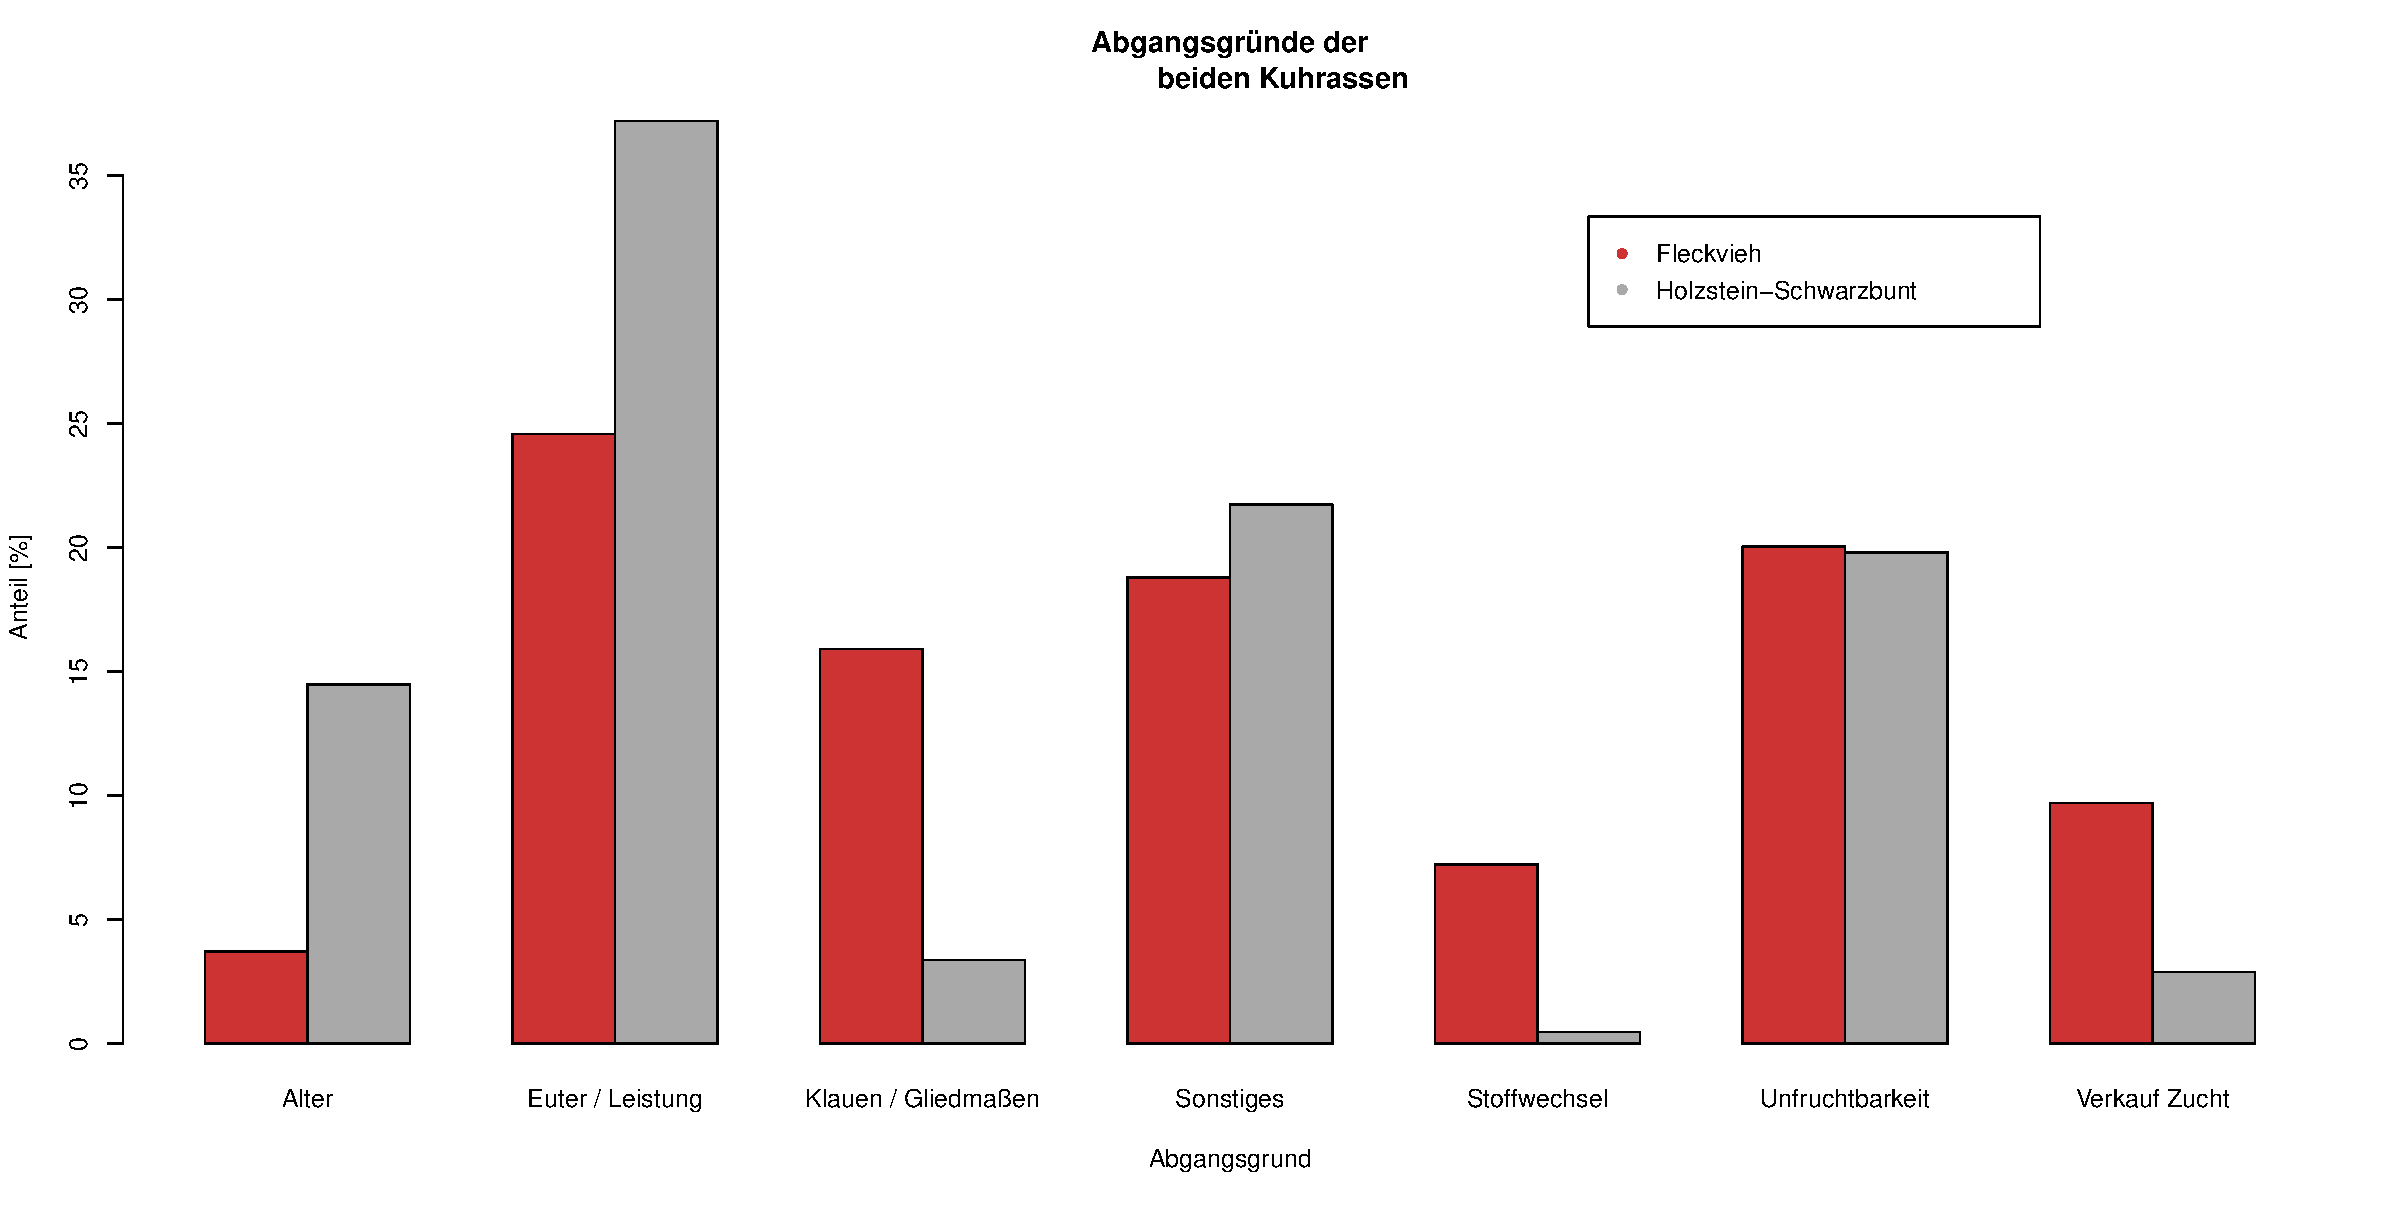
\includegraphics[scale = 0.32]{abgang.pdf}
			\caption{Säulendiagramme zu den Abgangsgründen der beiden Kuhrassen}
		\end{figure}
	\end{frame}
	
	\section{Laktationseinflüsse}
	\begin{frame}
		\frametitle{Laktationseinflüsse}
		\begin{figure}[htbp]
			\centering
			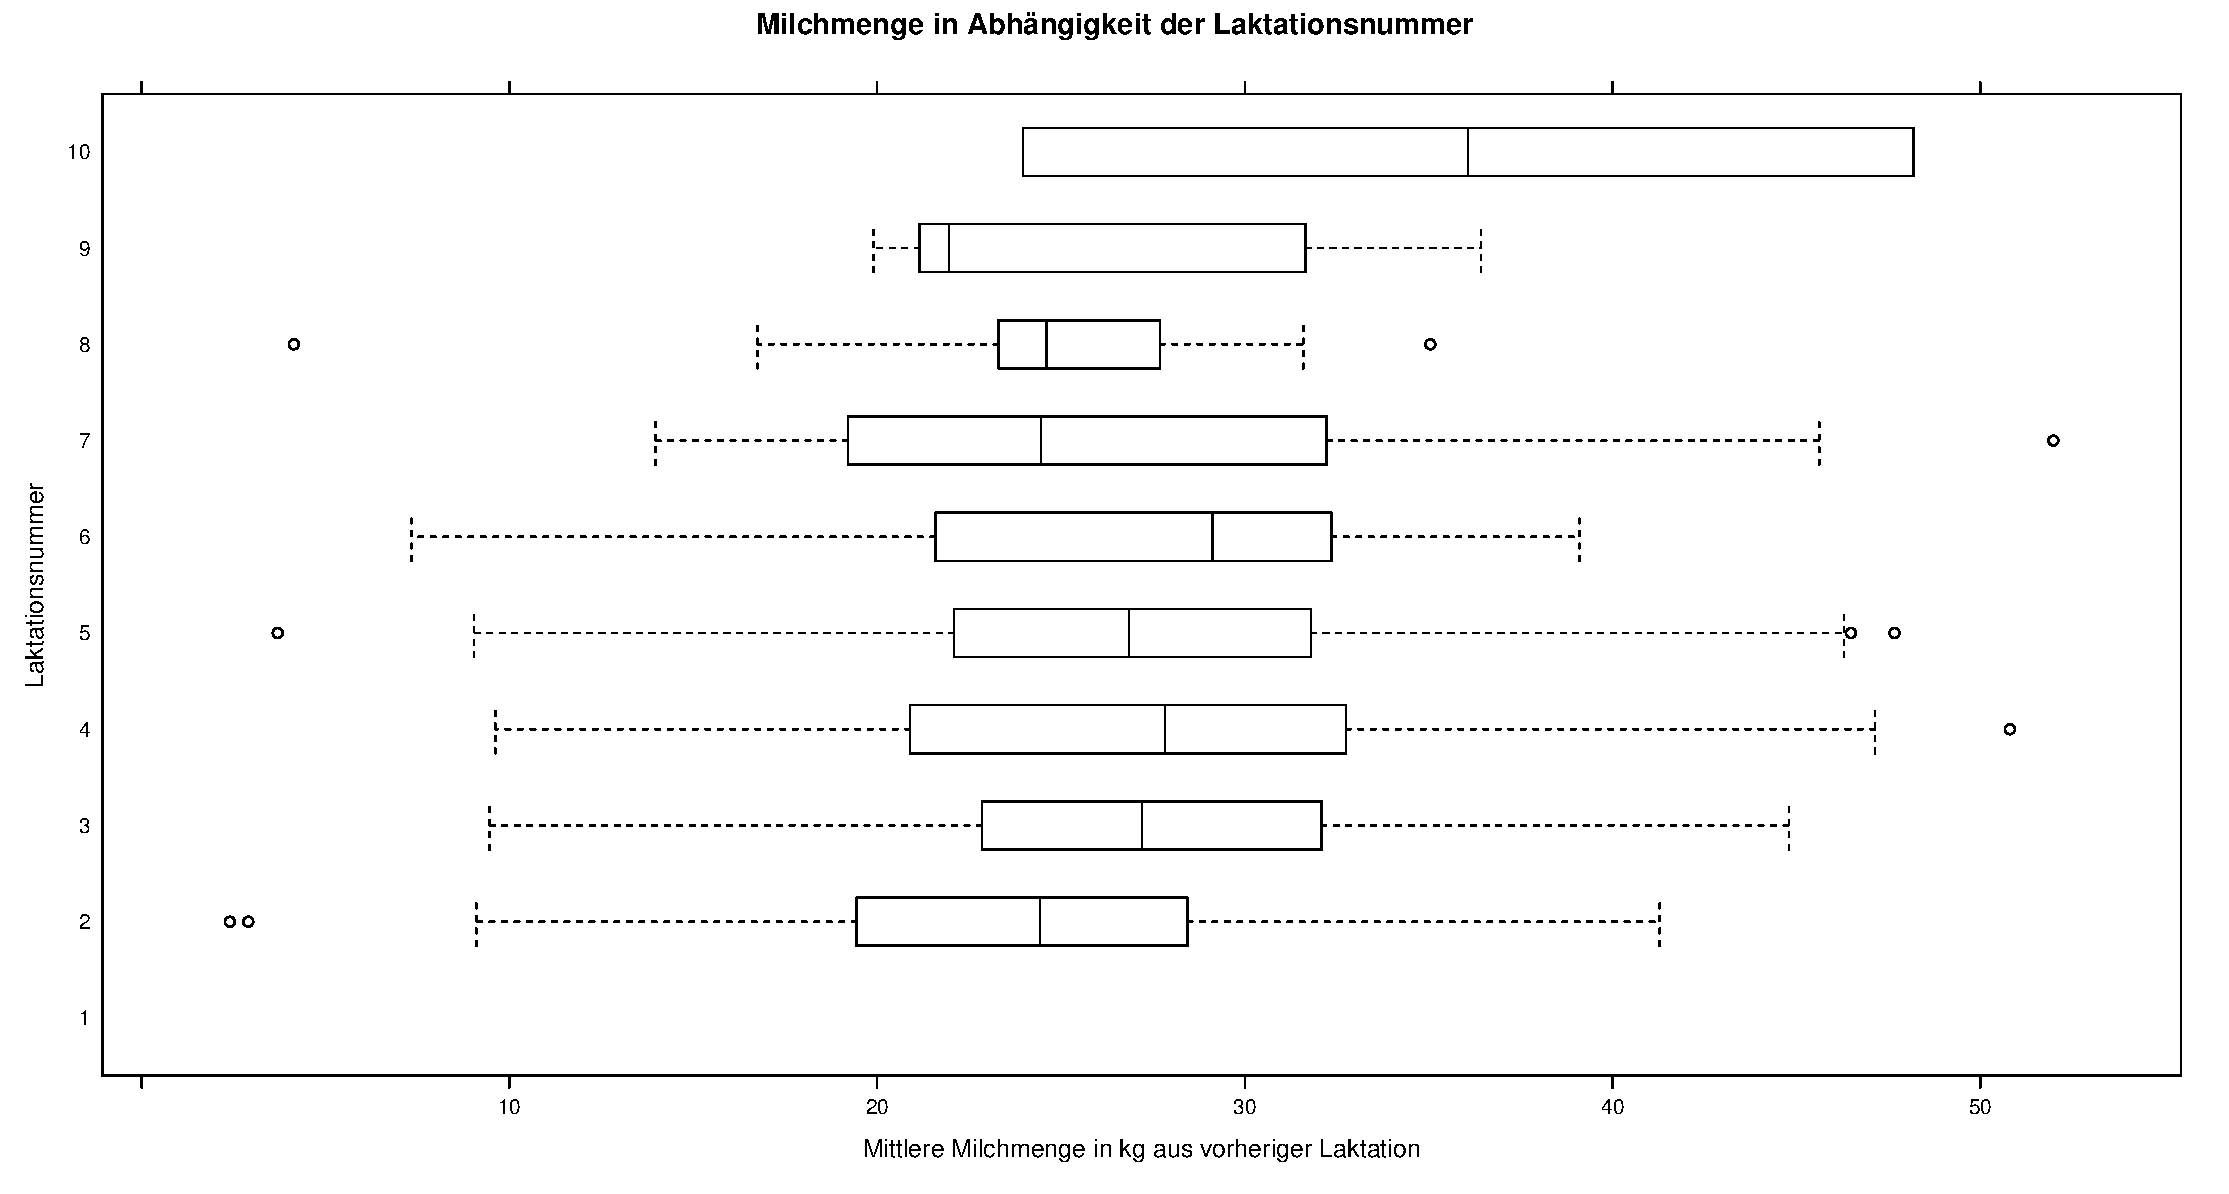
\includegraphics[scale = 0.333]{lattice.pdf}
			\vspace{-0.6cm}
			\caption{Boxplots zur Gegenüberstellung der Milchmenge und der aktuellen Laktationsnummer}
		\end{figure}
	\end{frame}

    	\section{Milchmenge und Gewicht}
	\begin{frame}
		\frametitle{Milchmenge und Gewicht}
		\begin{figure}[h]
			\centering
			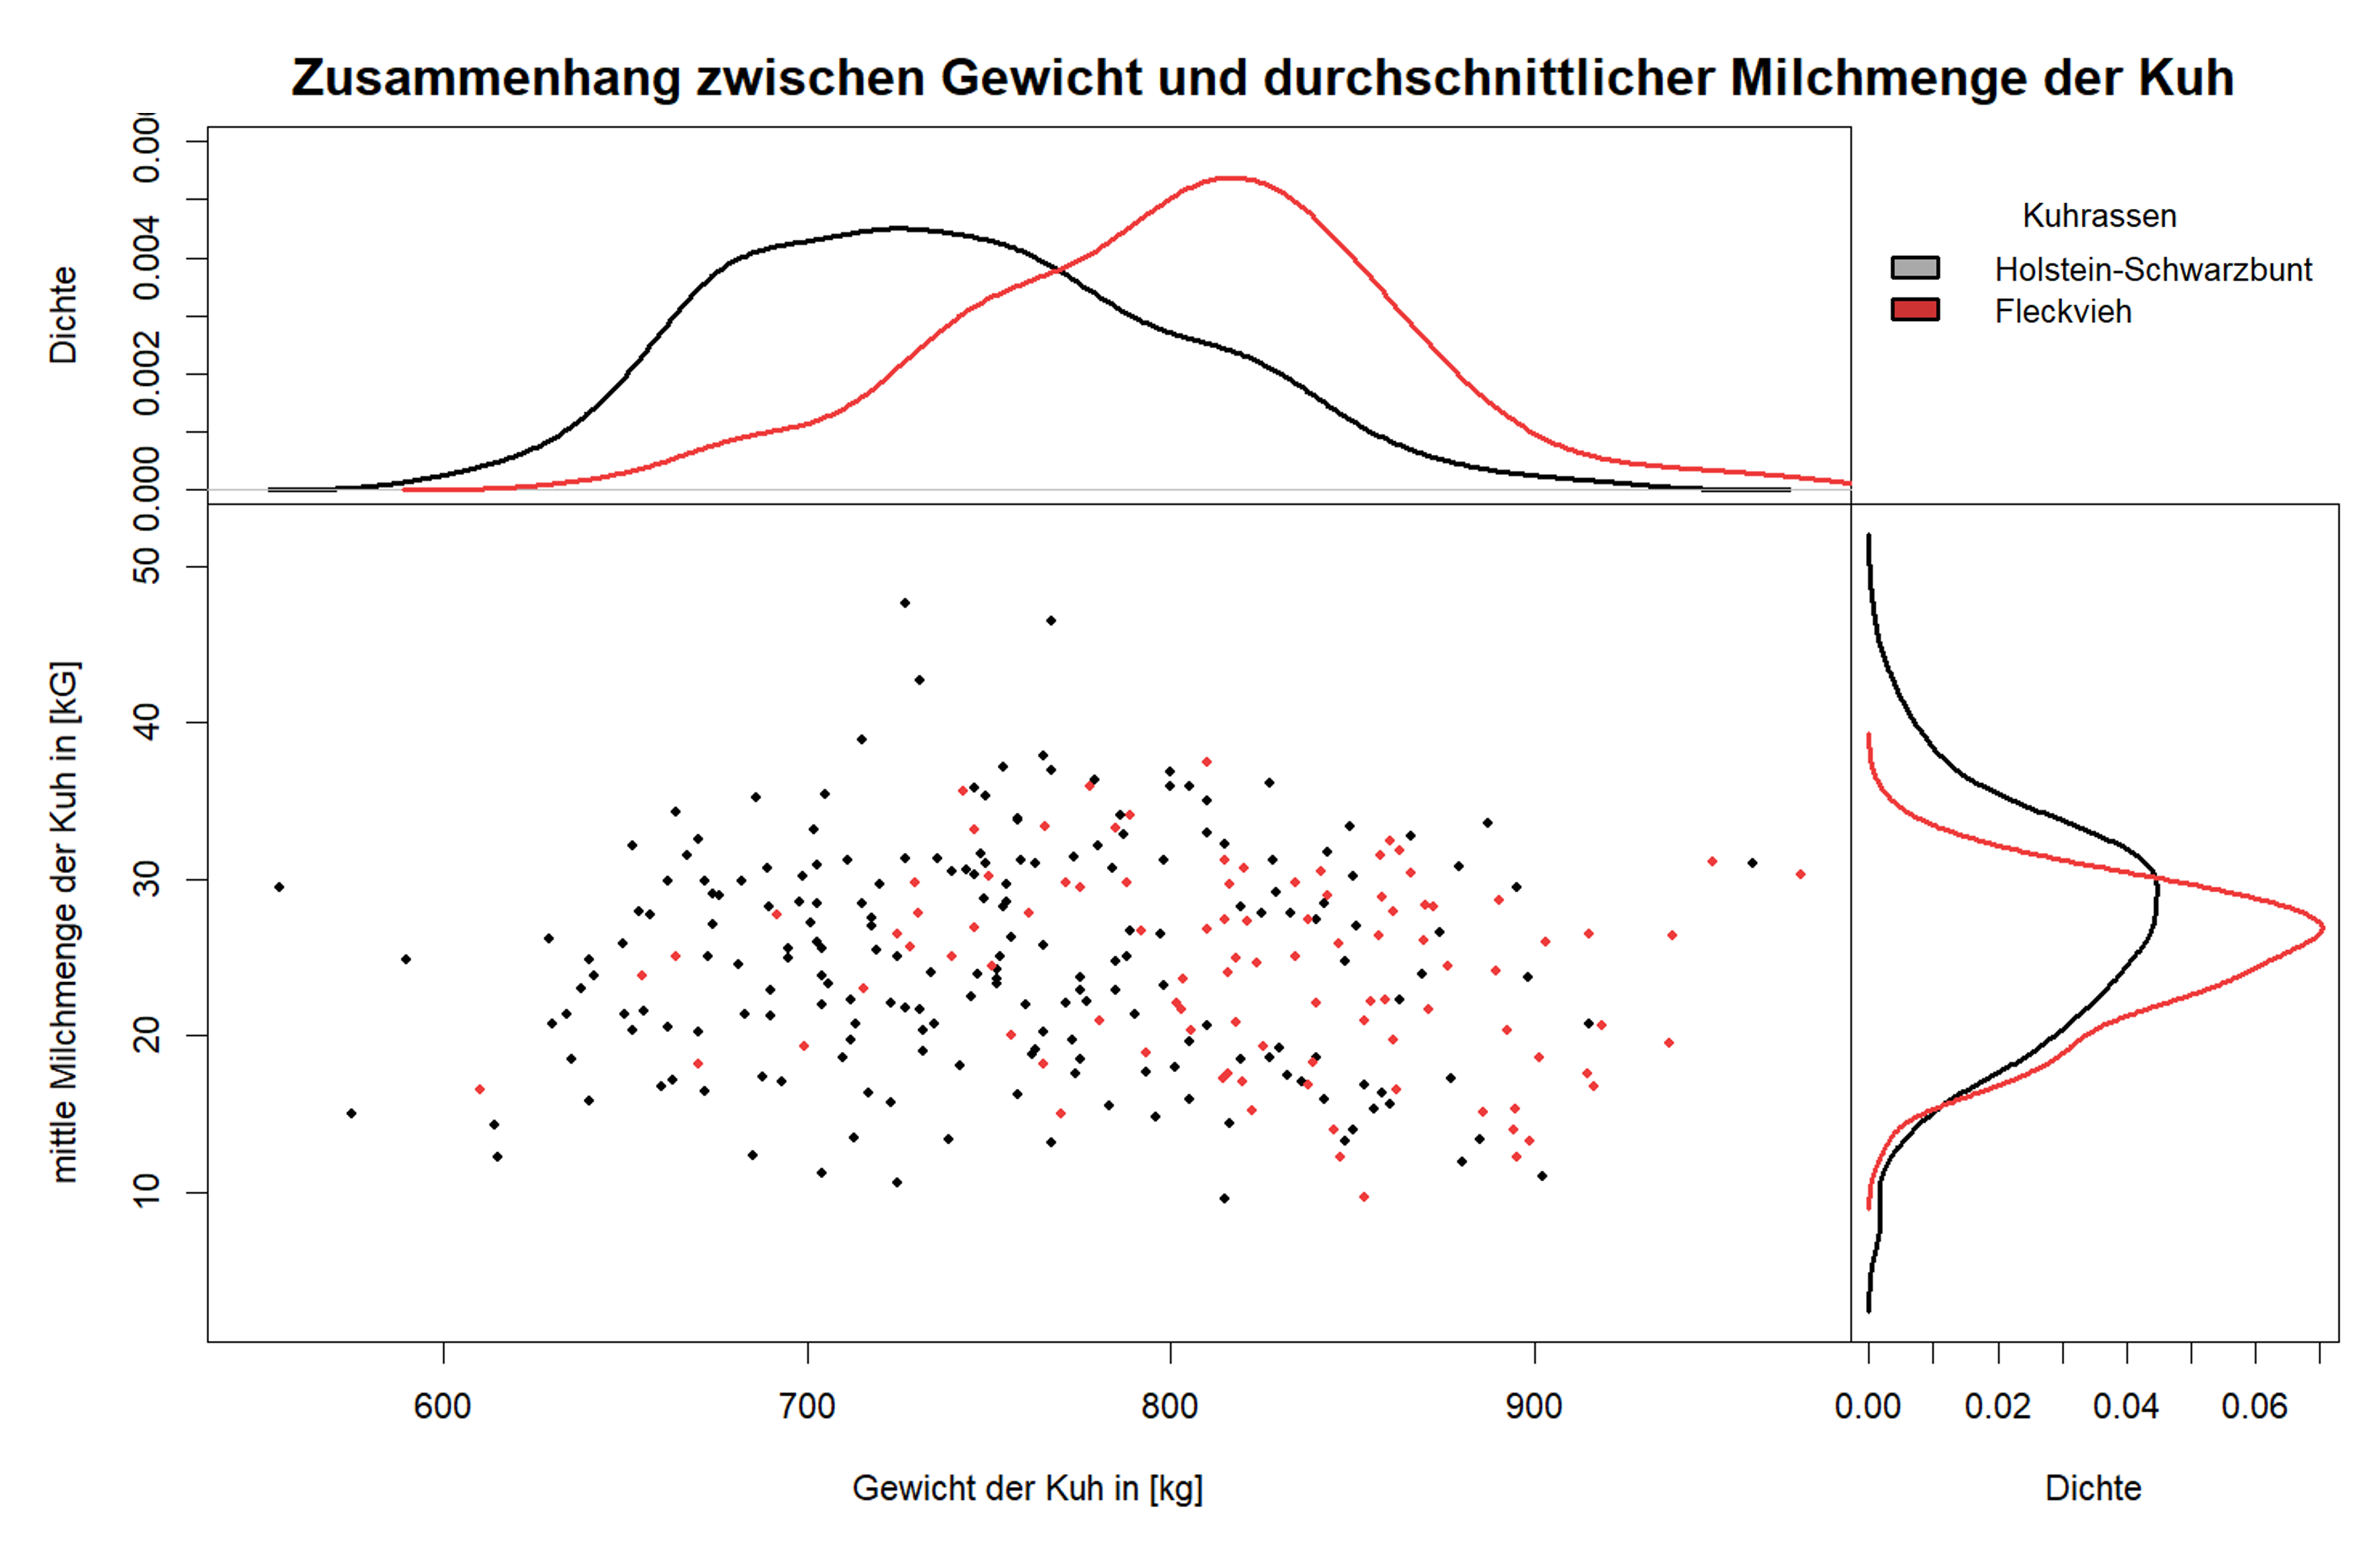
\includegraphics[width=1\textwidth]{Scatter und Kerndichte Milchmenge~Gewicht.png}
			\vspace{-0.6cm}
			\caption{Scatterplot und Kerndichten zur Gegenüberstellung der Milchmenge und des Gewichts}
		\end{figure}
	\end{frame}

    	\section{Milchmenge je Farm}
	\begin{frame}
		\frametitle{Milchmenge je Farm}
		\begin{figure}[h]
			\centering
			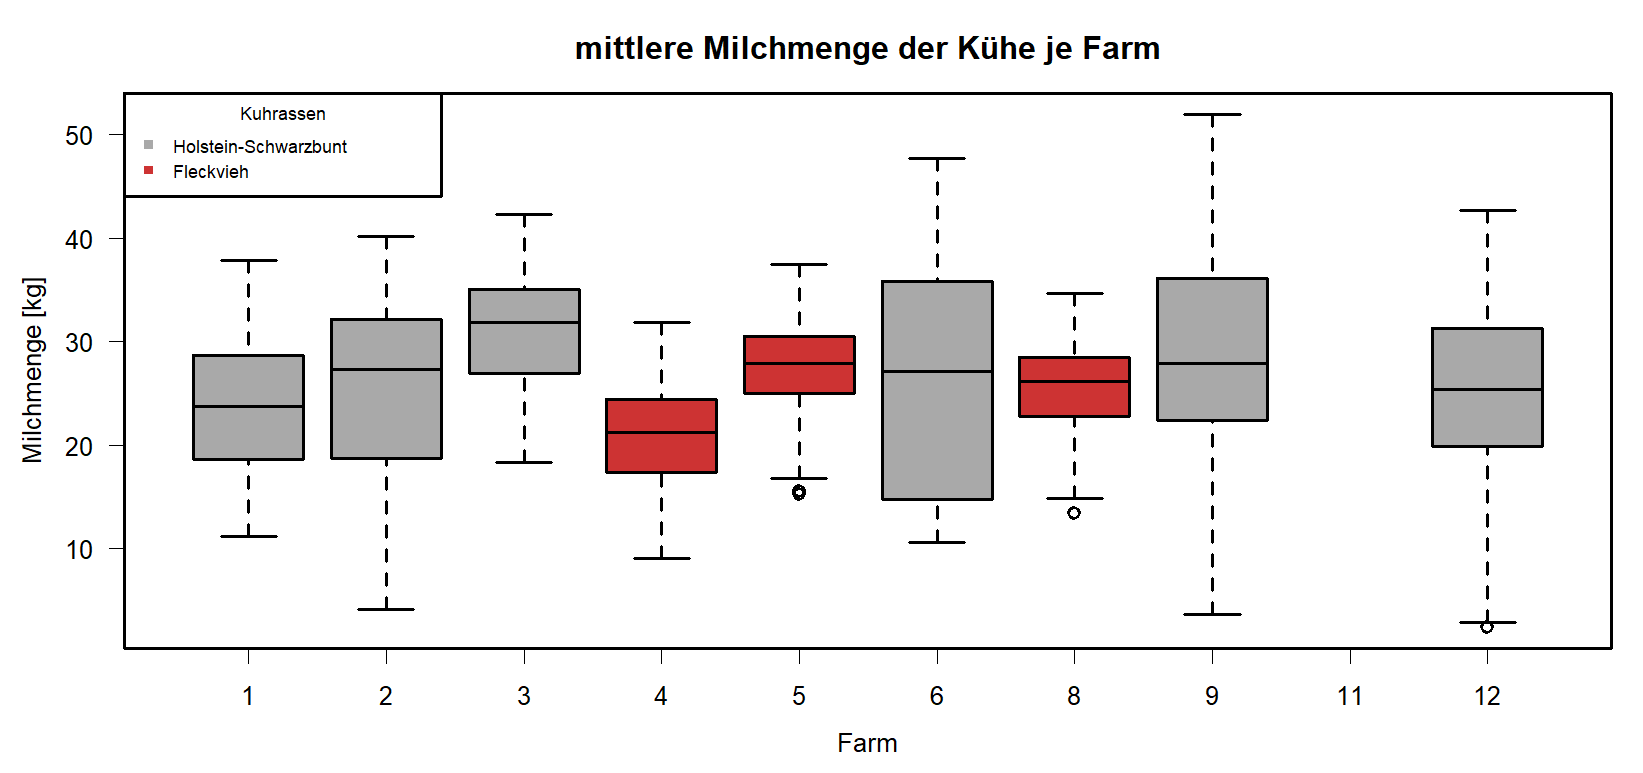
\includegraphics[width=1\textwidth]{Boxplot Milch~Farm.png}
			\vspace{-0.6cm}
			\caption{Boxplots zur mittleren durchschnittlichen Milchmenge je Farm}
		\end{figure}
	\end{frame}
	\begin{frame}
		\frametitle{Mosaikplot zur Krankheitsanzahl nach Rasse}
		\begin{figure}[h]
			\centering
			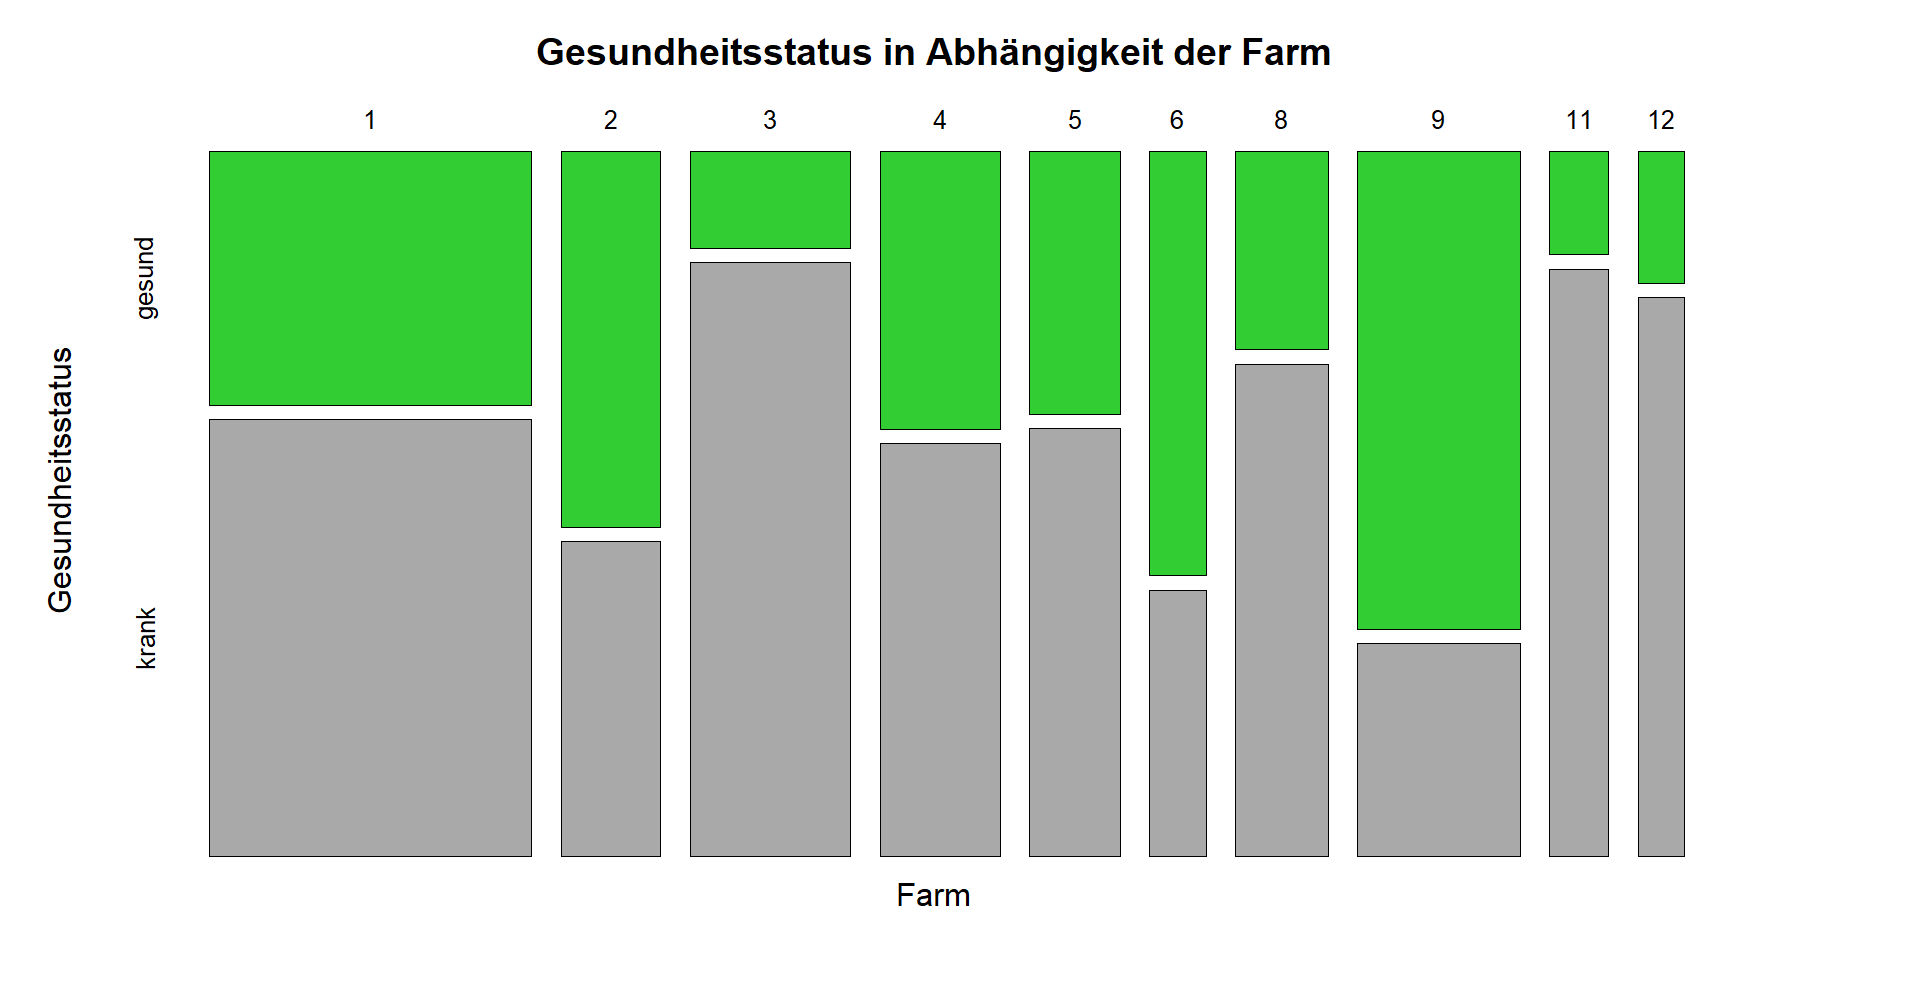
\includegraphics[scale=0.35]{Mosaikplots.png}
			\vspace{-0.6cm}
			\caption{Mosaikplot zur Krankheitsanzahl nach Rasse}
		\end{figure}
	\end{frame}
	\begin{frame}
		\frametitle{Bedingtes Dichtediagramm zu den Glukosewerten}
		\begin{figure}[h]
			\centering
			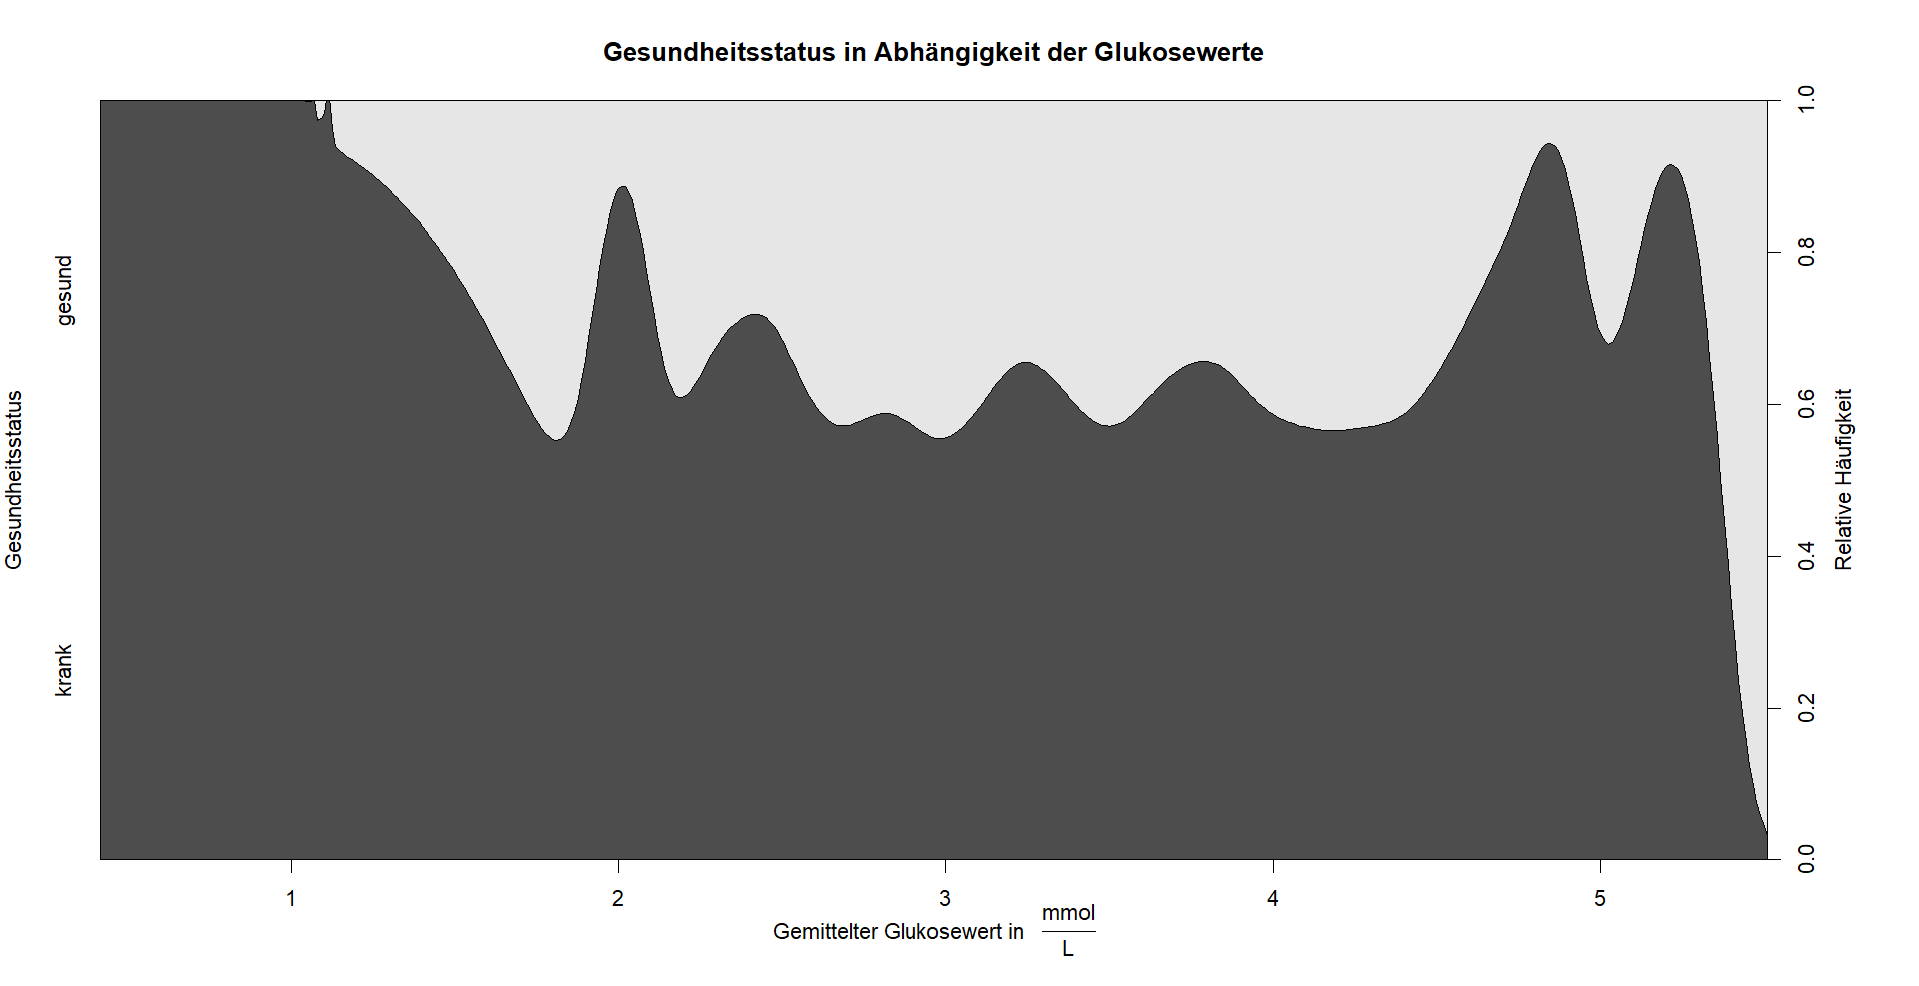
\includegraphics[scale=0.33]{Bedingtes Dichtediagramm.png}
			\vspace{-0.6cm}
			\caption{Bedingtes Dichtediagramm: Abhängigkeit Gesundheitsstatus  und Glukoswert}
		\end{figure}
	\end{frame}
	\begin{frame}
		\frametitle{Chernoff-Gesichter zu den Rassen}
	\begin{figure}[h]
		\centering
		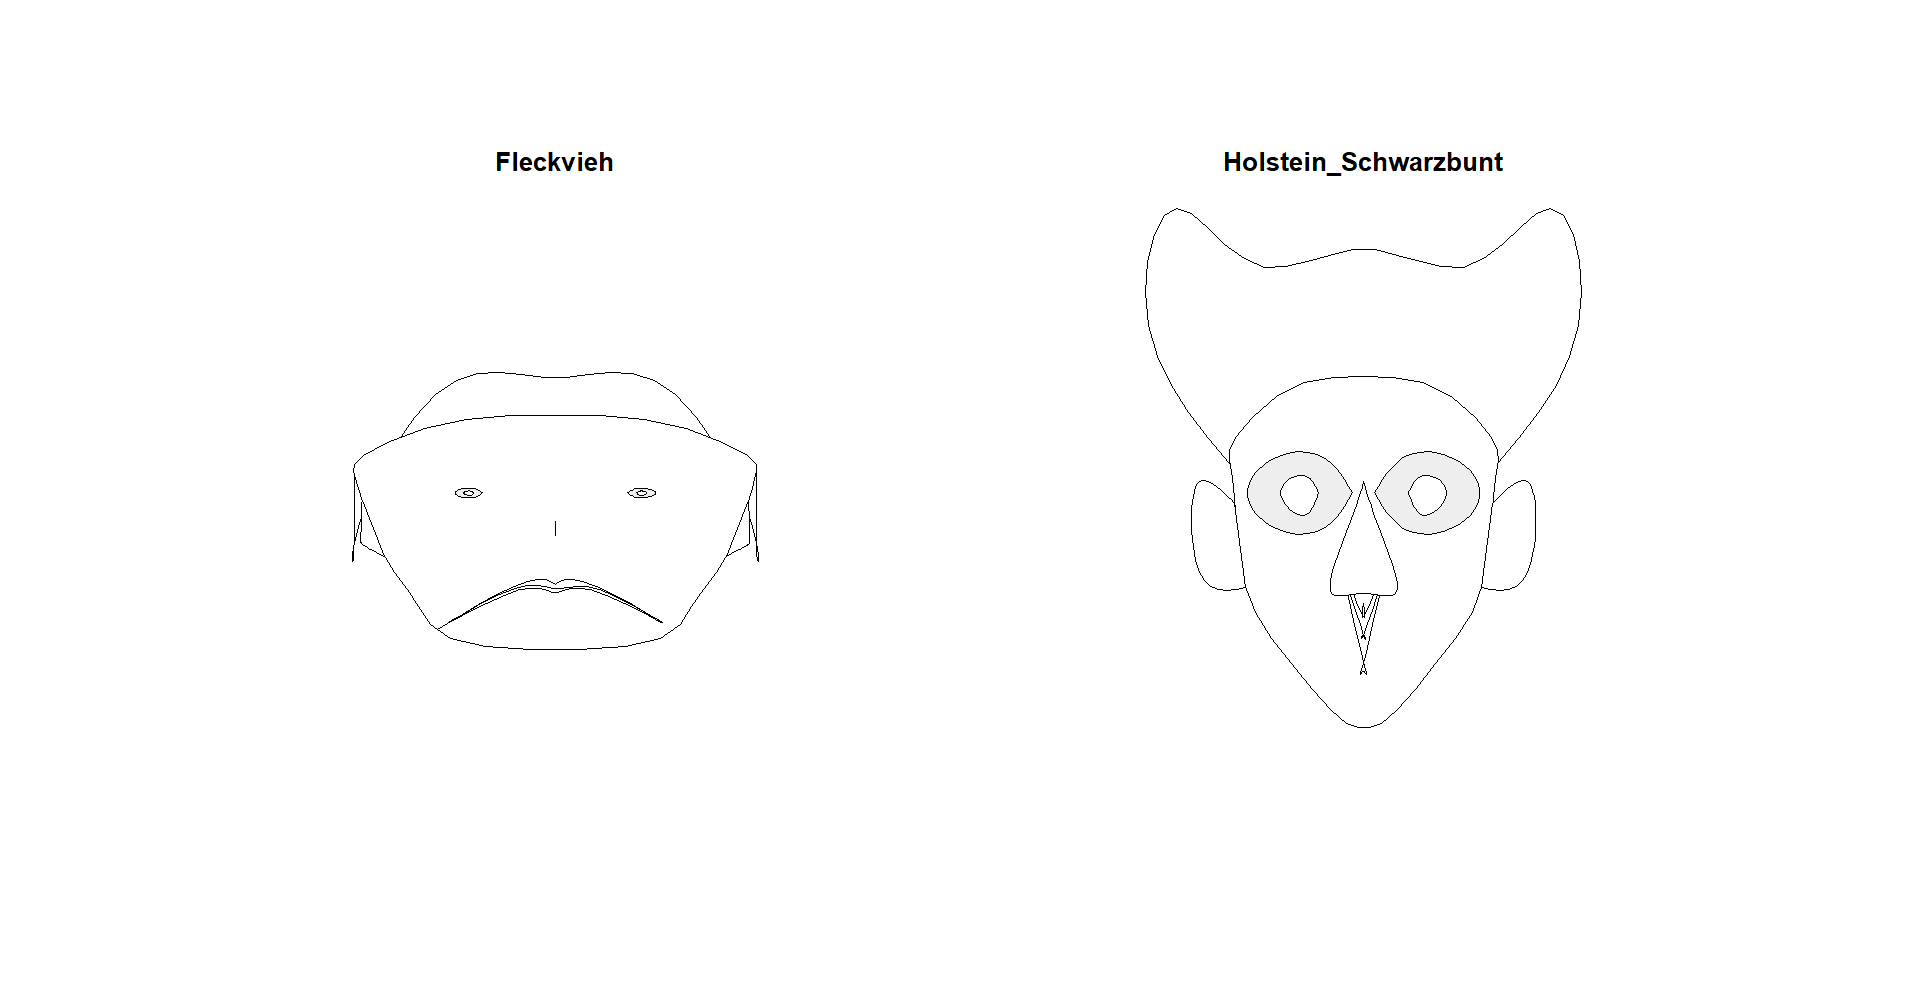
\includegraphics[width=1\textwidth]{Chernoff-Gesichter.png}
		\vspace{-0.6cm}
		\caption{Chernoff-Gesichter zu den Rassen anhand von 14 Variablen}
	\end{figure}
	\end{frame}
	
	\setbeamertemplate{footline}{%
		\leavevmode%
		\hbox{%
			\begin{beamercolorbox}[wd=.333333\paperwidth,ht=2.25ex,dp=1ex,left]{author in head/foot}%
				\usebeamerfont{author in head/foot}\insertshortauthor
			\end{beamercolorbox}%
			\begin{beamercolorbox}[wd=.333333\paperwidth,ht=2.25ex,dp=1ex,center]{title in head/foot}%
				\usebeamerfont{title in head/foot}\insertshorttitle
			\end{beamercolorbox}%
			\begin{beamercolorbox}[wd=.333333\paperwidth,ht=2.25ex,dp=1ex,right]{date in head/foot}%
				\usebeamerfont{date in head/foot}\hspace*{2em}
		\end{beamercolorbox}}%
		\vskip0pt%
	}
\begin{frame}
	\section{Literaturverzeichnis}
	\frametitle{Literaturverzeichnis}
	\begin{enumerate}[]
		\item Sarkar D (2008). \_Lattice: Multivariate Data Visualization with R\_.
		Springer, New York. ISBN 978-0-387-75968-5,
		<http://lmdvr.r-forge.r-project.org>.
		\item Signorell A (2024). \_DescTools: Tools for Descriptive Statistics\_. R package
		version 0.99.54, <https://CRAN.R-project.org/package=DescTools>.
	\end{enumerate}
	
\end{frame}
\end{document}
